% Created 2009-05-08 Fri 15:22
\documentclass[notes=hide]{beamer}
\usepackage[utf8]{inputenc}
\usepackage[T1]{fontenc}
\usepackage{hyperref}
\usepackage[english]{babel}
\usepackage{apacite} % after babel
\usepackage{natbib}
\usepackage{pslatex}
\pdfoutput=1

\usepackage{enumerate}
\usepackage{subfigure}
\usepackage{linguex}

\usepackage{color}
\usepackage{xcolor}

\usepackage{graphicx}       % for \includegraphics, only works when {cslipubs} is [FINAL]
\usepackage{amssymb}        % for \square

\usetheme{Goettingen}
%\setbeameroption{show notes}

\newcommand{\ana}[1]{\texttt{#1}}
\newcommand{\form}[1]{`#1'}
\newcommand{\tool}[1]{\texttt{#1}}
\newcommand{\fn}[1]{$\mathrm{#1}$}

\title[lt-trim]{FST Trimming: Ending Dictionary Redundancy in Apertium}
\author{Matthew Marting\inst{1} \and Kevin Unhammer\inst{2}}
\date{27th May 2014}
\institute[apertium]{
  \inst{1} St. David's School \\ Raleigh, NC. \\ {\tt \tiny $\emptyset{}$}
  \and
  \inst{2} Kaldera språkteknologi \\ Stavanger, Noreg \\ {\tt \tiny unhammer+apertium@mm.st}
}

\begin{document}
\maketitle


\begin{frame}
  \frametitle{Outline of talk}
  \note{}
\setcounter{tocdepth}{1}
\tableofcontents[] % add pausesections? (one slide per \section)
\setcounter{tocdepth}{3}
\end{frame}

\section{Introduction and background}
\begin{frame}\frametitle{Introduction and background}
  \note{}
  \begin{itemize}
    \item Apertium: Free/Open Source, Rule-based Machine Translation platform
    \item Goals include:
      \begin{itemize}
      \item supporting lesser-resourced languages
      \item wide coverage
      \item post-editable output
      \item reusable resources
      \end{itemize}
    \item Language data (dictionaries, etc.) typically organised in
      language \emph{pairs} (Catalan-Spanish, Portuguese-Spanish,
      etc.)
      \begin{itemize}
      \item historically: each with its own copy of monolingual data
      \end{itemize}
  \end{itemize}
\end{frame}

\begin{frame}[plain]
  \begin{figure}[h]
    \begin{center}
      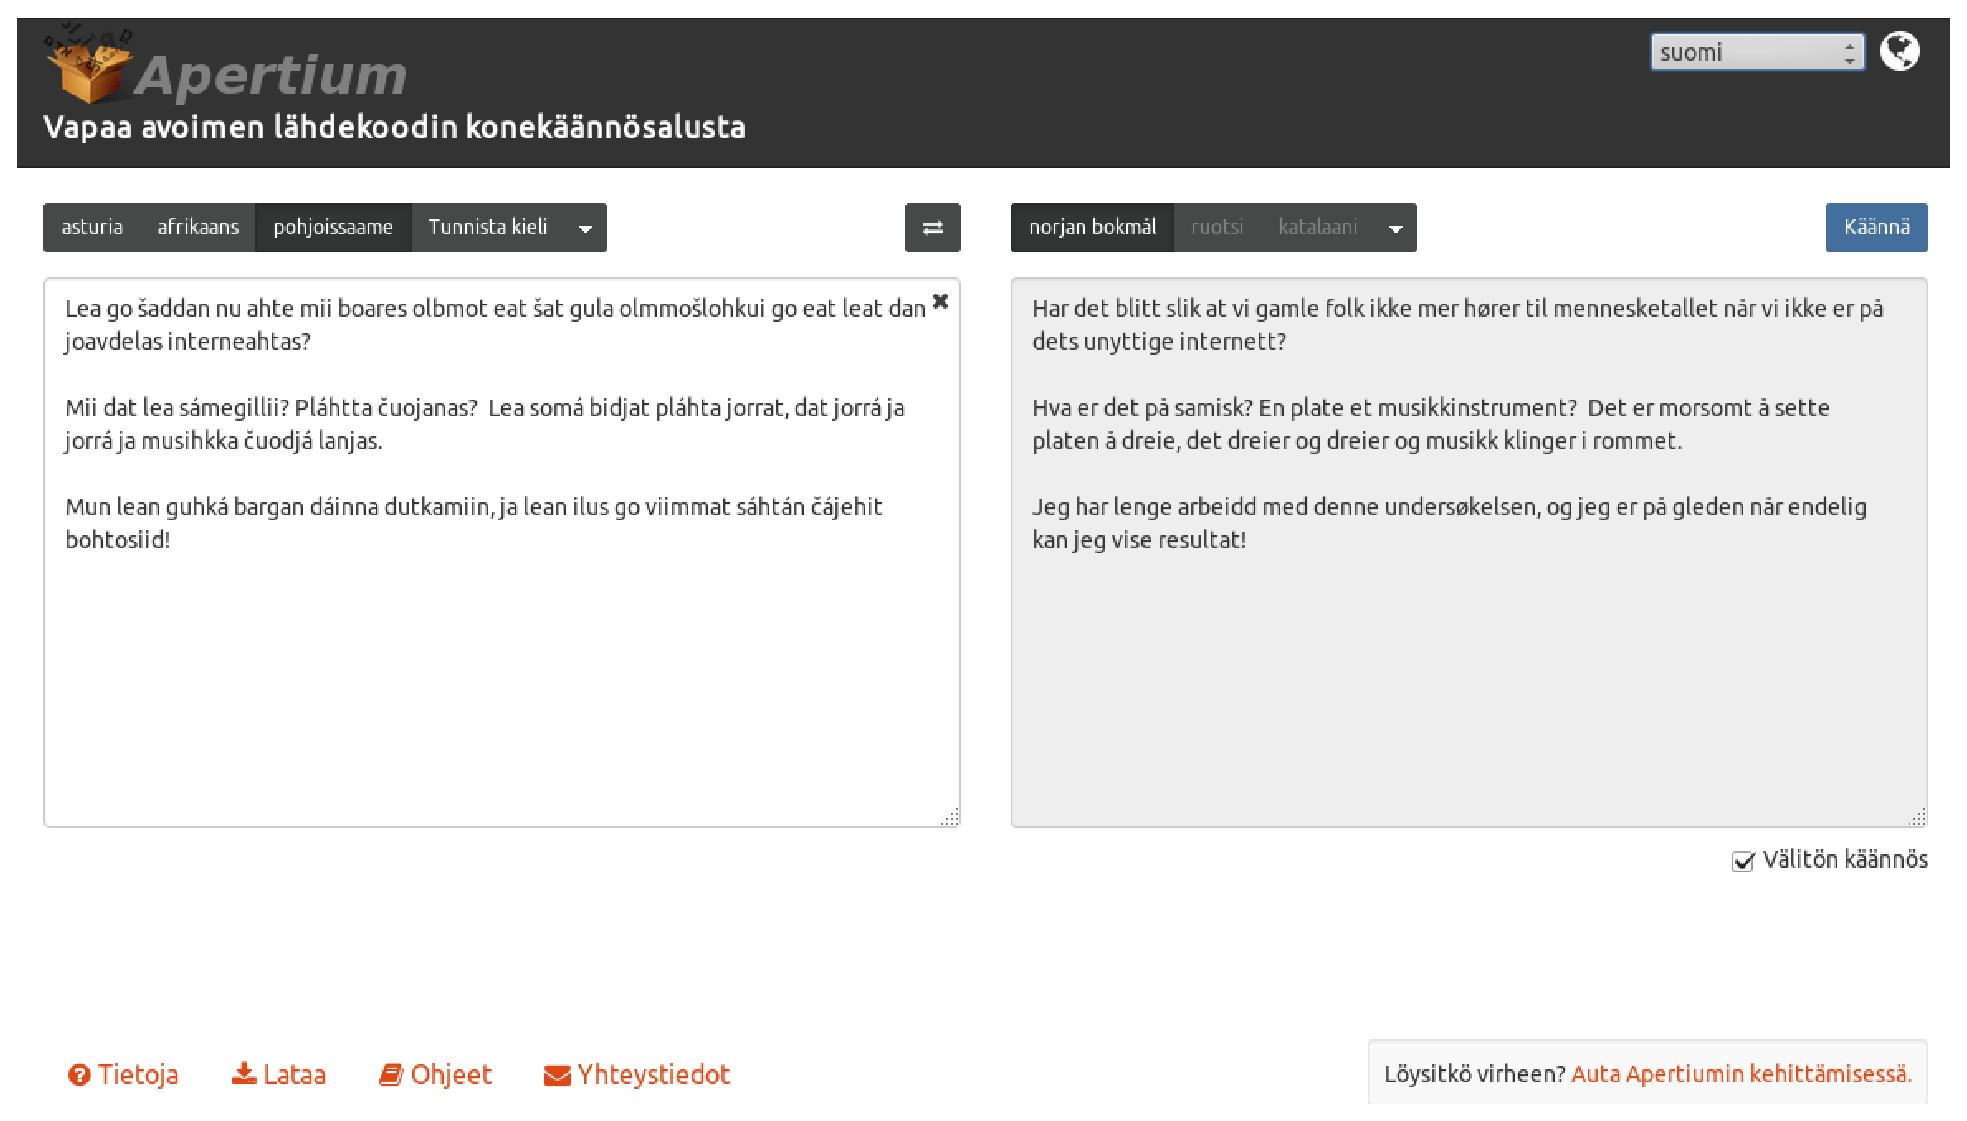
\includegraphics[scale=0.35]{apertium-www.eps}
    \end{center}
  \end{figure}
\end{frame}


\subsection{FST's in the Apertium pipeline}
\begin{frame}
  \frametitle{Apertium pipeline architecture}
  \begin{itemize}
    \item lttoolbox Finite State Transducers used for, among others:
      \begin{itemize}
      \item morph. analysis: \form{fishes} to \ana{fish<n><pl>/fish<vblex><pres>}
      \item lex. transfer: \ana{fish<n><pl>} to \ana{fisk<n><m><pl>}
      \item morph. generation: \ana{fisk<n><m><pl><def>} to \form{fiskane}
      \end{itemize}
  \end{itemize}
  \begin{figure}[h]
    \begin{center}
      \includegraphics[scale=0.8]{architecture.eps}
    \end{center}
  \end{figure}
\end{frame}

\begin{frame}
  \frametitle{Multiword support}
  lttoolbox FST's support a variety of multiwords

  ~ \\

  An lttoolbox ``lexical unit'' is one token, and can be:
  \begin{itemize}
  \item simple non-multi-words: \form{fish}
  \item simple space-separated words: \form{hairy frogfish} as a
    single token
  \item multiwords with \textbf{inner inflection}: \form{takes out}, \\
    analysed as \ana{take<vblex><pri><p3><sg>\# out},\\
    converted to \ana{take\# out<vblex><pri><p3><sg>} before lexical
    transfer
  \end{itemize}
\end{frame}

\begin{frame}
  \frametitle{Multiword support}

  \begin{itemize}
  \item \textbf{joined} multiwords: \form{they'll}; \\
    analysed as single token \ana{prpers<prn><subj><p3><mf><pl>+will<vaux><inf>}, \\
    then split into two tokens \ana{prpers<prn><subj><p3><mf><pl>} and
    \ana{will<vaux><inf>} before lexical transfer
  \item \textbf{compounds}: \form{frogfish}; \\
    analysed as single token \ana{frog<n><sg>+fish<n><pl>}, \\
    then split into two tokens \ana{frog<n><sg>} and \ana{fish<n><pl>}
    before lexical transfer
  \end{itemize}
\end{frame}

\begin{frame}
  \frametitle{Multiword support}
  \begin{itemize}
  \item combinations (space-separated + joined + inner inflection):
    \form{creure-ho que},\\
    analysed as single token \ana{creure<vblex><inf>+ho<prn><enc><p3><nt>\# que}, \\
    then moved and split into two tokens \\
    \ana{creure\# que<vblex><inf>} and \ana{ho<prn><enc><p3><nt>}
    before lexical transfer
  \end{itemize}
\end{frame}

\subsection{The Problem: Redundant data}
\begin{frame}
  \frametitle{The Problem: Redundant data}

  \begin{center}
    \begin{figure}[h]
      \includegraphics[scale=0.6]{../pairs-after.eps}
    \end{figure}
    \small{Ideal number of monodixes with four languages}

    \begin{figure}[h]
      \includegraphics[scale=0.6]{../pairs-before.eps}
    \end{figure}
    \small{Current number of monodixes with pairs of four languages}
  \end{center}

\end{frame}

\begin{frame}
  Words in analyser but missing from lexical transfer can be
  problematic:
  \begin{itemize}
  \item \form{fishes} to \form{@fish}: loses the inflection
  \item \form{gikk til hundene} ``went to the dogs'' to
    \form{went to @hund} ``went to dog'': losing the
    inflection hides the idiomatic meaning
  \item \form{öldürmedi} ``did not kill'' to \form{@öl} ``kill'':
    loses the \emph{negation}
  \item lexical transfer is also tag transfer – structural transfer
    thus needs exceptions for half-translated tags
  \end{itemize}
\end{frame}

\begin{frame}
  But, most importantly, multiword tokenisation means that

  ~

  \form{He takes out the trash} translates to \form{Han @take out
    søpla} \emph{even though both \form{take}-\form{ta} and
    \form{out}-\form{ut} are in the bilingual dictionary}.

  ~

  Adding more words makes the translator worse!
\end{frame}

\subsection{A Solution: trim on compile}
\begin{frame}
  \frametitle{A Solution: trim on compile}
  Compile a \emph{trimmed} analyser-FST containing only those entries
  from original analyser FST that would pass through bilingual FST.

  ~\\

  \begin{itemize}
  \item FSA's closed under intersection: FSA1 $\cap$ FSA2 = FSA3
  \item Similarly, we can compose-intersect FST's:\\
    output-side of FST1 $\cap$ input-side of FST2 = FST3
  \end{itemize}

  ~\\

  Goal: One big monolingual source dictionary, trimmed during compile
  to language-pair specific analysers.

  Dictionaries in HFST instead of lttoolbox can trim already (but it
  breaks with compounds!).

  Most Apertium dictionaries use lttoolbox.


\end{frame}

\begin{frame}
  Our tool needs some exceptions to compose-intersect:
  \begin{itemize}
  \item Append $.*$ (any-symbol loop) to bilingual FST
    \begin{itemize}
    \item Lexical transfer only needs a match on the start of the
      string
    \end{itemize}

  \item Reorder \ana{\#}-multiwords in bilingual FST
    \begin{itemize}
    \item so they look like analyser (else they won't match)
    \end{itemize}

  \item Let \ana{+} in analyser mean transition-to-start in bilingual
    FST
    \begin{itemize}
    \item since single token \ana{a+b} in analyser is split into two
      tokens \ana{a} \ana{b} before lexical transfer
    \end{itemize}

  \end{itemize}
\end{frame}

\begin{frame}
  Digression: Some Apertium dictionaries use HFST instead of
  lttoolbox.

  ~\\

  Trimming with standard HFST commands works for most but not all such
  dictionaries.

  ~\\

  Again multiword issues: compounds.
\end{frame}

\section{Implementation of \tool{lt-trim}}
\begin{frame}
  \frametitle{Implementation of \tool{lt-trim}}
  Tool takes two compiled FST's, produces a new, \emph{trimmed} FST
  \begin{enumerate}
  \item Preprocess bilingual FST
    \begin{enumerate}
    \item ``Prefixing'': Append any-symbol loop
    \item Reorder \#-multiwords
    \end{enumerate}
  \item Depth-first intersection of output-side of analyser with
    input-side of bilingual FST
    \begin{itemize}
    \item with an exception on seeing +
    \end{itemize}
  \end{enumerate}
\end{frame}

\subsection{Preprocessing the bilingual dictionary}
\begin{frame}
  \frametitle{Prefixing bilingual FST}
  \begin{center}
    \begin{figure}[h]
      \includegraphics[scale=0.6]{bi.eps}
    \end{figure}
    \scriptsize{Input bilingual FST (letter transitions compressed to single arcs)}
    \begin{figure}[h]
      \includegraphics[scale=0.6]{bi-prefixed.eps}
    \end{figure}
    \scriptsize{``Prefixed'' bilingual FST (any-symbol loop appended)}
  \end{center}
\end{frame}

\begin{frame}
  \frametitle{Moving uninflected lemma parts in bilingual FST}
  Want \ana{take\# out<vblex>} to become \ana{take<vblex>\# out}, so 
  \begin{enumerate}
  \item Depth-first traverse bilingual FST
  \item On seeing a \#, replace the transition $t$ with results of \fn{copyWithTagsFirst(t)}
  \item Function \fn{copyWithTagsFirst(t)} builds a new partial FST
    where any tag sequence and uninflected lemma parts have swapped
    places
  \end{enumerate}
\end{frame}

\begin{frame}
  \frametitle{Moving uninflected lemma parts in bilingual FST}
  \begin{center}
    \begin{figure}[h]
      \includegraphics[scale=0.7]{bi-prefixed.eps}
    \end{figure}

    \begin{figure}[h]
      \includegraphics[scale=0.7]{bi-prefixed-moved.eps}
    \end{figure}
  \end{center}

\end{frame}


\subsection{Intersection}

\begin{frame}
  \frametitle{Intersection}
  \begin{center}
    \begin{figure}[h]
      \includegraphics[scale=0.6]{mono-simple.eps}
    \end{figure}
    \scriptsize{Input analyser}
    \begin{figure}[h]
      \includegraphics[scale=0.6]{bi-prefixed-moved.eps}
    \end{figure}
    \scriptsize{Preprocessed bilingual FST}
  \end{center}
\end{frame}

\begin{frame}
  \begin{center}
    \begin{figure}[h]
      \includegraphics[scale=0.6]{trimmed-simple-1.eps}
    \end{figure}
  \end{center}
\end{frame}

\begin{frame}
  \begin{center}
    \begin{figure}[h]
      \includegraphics[scale=0.6]{trimmed-simple-2.eps}
    \end{figure}
  \end{center}
\end{frame}

\begin{frame}
  \begin{center}
    \begin{figure}[h]
      \includegraphics[scale=0.6]{trimmed-simple-3.eps}
    \end{figure}
  \end{center}
\end{frame}

\begin{frame}
  \begin{center}
    \begin{figure}[h]
      \includegraphics[scale=0.6]{trimmed-simple-4.eps}
    \end{figure}
  \end{center}
\end{frame}

\begin{frame}
  \begin{center}

    \begin{figure}[h]
      \includegraphics[scale=0.7]{mono-simple.eps}
    \end{figure}
    \scriptsize{Input analyser}

    \begin{figure}[h]
      \includegraphics[scale=0.7]{trimmed-simple.eps}
    \end{figure}
    \scriptsize{Fully trimmed analyser}

  \end{center}
\end{frame}

\begin{frame}
  \frametitle{Intersection with multiwords}
  \begin{center}
    \begin{figure}[h]
      \includegraphics[scale=0.6]{mono.eps}
    \end{figure}
    \scriptsize{Input analyser}

    \begin{figure}[h]
      \includegraphics[scale=0.6]{trimmed.eps}
    \end{figure}
    \scriptsize{Trimmed analyser}
  \end{center}
\end{frame}

\subsection{\tool{lt-trim} in use}
\begin{frame}
  \frametitle{\tool{lt-trim} in use}
  \tool{\$ lt-trim full-ana.bin bi.bin trimmed-ana.bin}

  ~\\

  (But language pair developers typically just type ``make''.)

  ~\\

  Speed and memory usage is comparable to regular lttoolbox
  (\tool{lt-comp}) compiling.
\end{frame}

\section{Ending Dictionary Redundancy}
\begin{frame}
  \frametitle{Ending Dictionary Redundancy}
  \begin{itemize}
  \item New Autotools rules let us formally depend on monolingual data
    packages
  \item All new languages added to Apertium use this system – no
    monolingual data redundancy
  \item But: Implementing trimming in old/well-developed language
    pairs means manual merging – divergent dictionaries problematic
    \begin{itemize}
    \item Merging Norwegian Bokmål between sme-nob and nno-nob: about
      3 hrs work
    \item dan-nob added further 3 hrs
    \end{itemize}
  \end{itemize}
\end{frame}

\section{Conclusion}
\begin{frame}
  \frametitle{Conclusion}
  \begin{itemize}
  \item \tool{lt-trim} works
  \item Monolingual data now in a single /languages/ SVN module,
    easier for other projects to find and use our data \\

  \item Next up: special-purpose HFST trimming tool to get around
    compounding problem?
  \item Still much manual merge work to be done
  \end{itemize}
\end{frame}

% TODO: Thanks for listening-slide? 


\end{document}
